\section{Desarrollo experimental 9}

\section{Desarrollo experimental 10}
 Para esta parte conectaremos un circuito auxiliar a la salida del generador de funciones:

 \begin{figure}[H]
    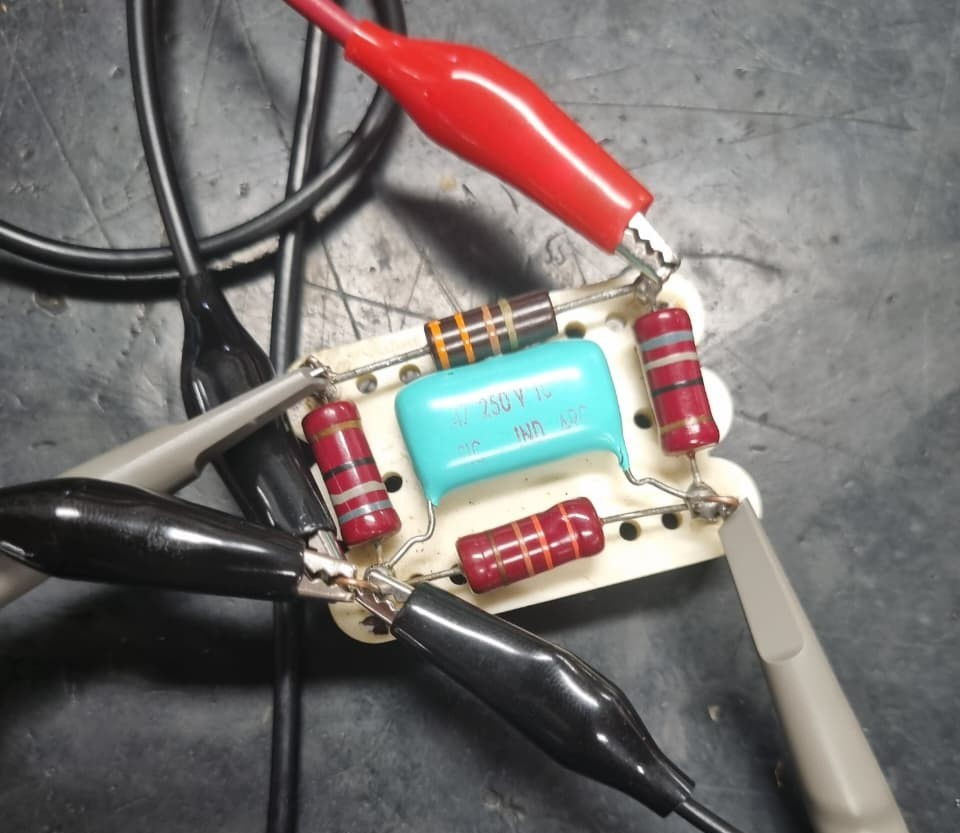
\includegraphics[width=0.4\textwidth]{images/parte10a.jpeg}
    \caption{Señal en x10 con acoplamiento en CA}
    \label{fig:calibracion}
\end{figure}

Y condiguramos el generador con los siguientes datos:

\begin{table}[H]
\resizebox{\columnwidth}{!}{%
\begin{tabular}{|c|c|c|c|c|}
\hline
\textbf{Frec.} & \textbf{Func.} & \textbf{Ampl.} & \textbf{Duty} & \textbf{Trig. on/off} \\ \hline
1KHz           & Cuadr.         & 10Vpp          & 20\%          & off                   \\ \hline
\end{tabular}%
}
\end{table}

Ahora pondremos el osciloscopio en modo "Dual", es decir doble canal. Ajustamos ambos canales a 0.2V/div, y la base de tiempo a 0.2ms/div, cambiamos a modo "Suma", y localizaremos el inversor del canal 2, para obtener lo siguiente:

\begin{figure}[H]
    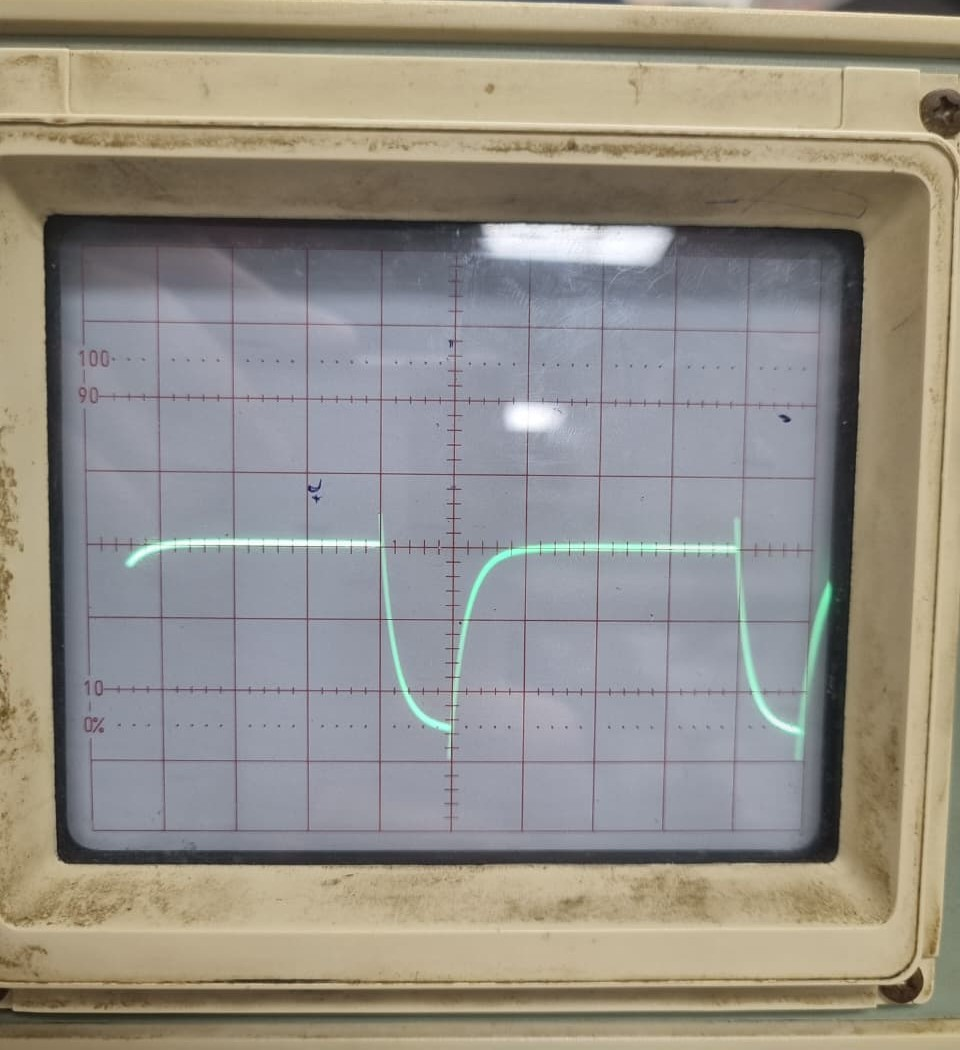
\includegraphics[width=0.4\textwidth]{images/parte10b.jpeg}
    \caption{Señal en x10 con acoplamiento en CA}
    \label{fig:calibracion}
\end{figure}

Y a partir de lo visto obtendremos los siguientes valores:

\begin{table}[H]
\resizebox{\columnwidth}{!}{%
\begin{tabular}{|l|l|l|l|l|}
\hline
V/div (Y1)                & V/div (Y2)               & T/div & Aten Y1                  & Aten Y2                  \\ \hline
\multicolumn{1}{|c|}{0.2V} & \multicolumn{1}{c|}{0.2V} & 0.2ms & \multicolumn{1}{c|}{x10} & \multicolumn{1}{c|}{x10} \\ \hline
\end{tabular}%
}
\end{table}

\begin{table}[H]
\resizebox{\columnwidth}{!}{%
\begin{tabular}{|c|c|c|c|c|c|}
\hline
\textbf{Período} & \textbf{Ancho} & \textbf{Ciclo Trab.} & \textbf{Vpp} & \textbf{Vcc} & \textbf{Vef} \\ \hline
1ms              & 0.64ms         & 0.64                 & 520mV        & 160mV        & 249.6mV      \\ \hline
\end{tabular}%
}
\end{table}

\section{Desarrollo experimental 11}